\chapter{Revisão da Literatura}
\label{cap:02}

% ============================================================
\section{Compatibilidade de Hardware como Domínio do Problema}
\label{sec:compatibilidade-hardware}
% ============================================================
A montagem de um computador \textit{desktop} exige o cruzamento de especificações técnicas entre componentes interdependentes.
Diferentemente da aquisição de periféricos genéricos, a configuração de um sistema computacional envolve restrições físicas, elétricas
e lógicas que, quando violadas, resultam em incompatibilidade absoluta: componentes adquiridos de forma incorreta não funcionam juntos,
independentemente de ajustes de \textit{software} ou configuração. Esse cenário impõe ao usuário leigo um desafio técnico significativo,
uma vez que plataformas comerciais tradicionais não oferecem mecanismos de validação preventiva capazes de explicar o motivo da incompatibilidade.

O presente trabalho concentra-se em cinco categorias de componentes que constituem o núcleo de qualquer configuração \textit{desktop}:
a Unidade Central de Processamento (CPU), a placa-mãe, os módulos de memória RAM, a Unidade de Processamento Gráfico (GPU) e a fonte de alimentação.
Cada uma dessas categorias possui especificações técnicas que determinam sua compatibilidade com as demais, formando uma rede de dependências
que não pode ser avaliada de forma isolada.

\subsection{Compatibilidade de Soquete CPU-Placa-mãe}
A restrição mais fundamental na montagem de um computador é a compatibilidade de soquete entre o processador e a placa-mãe.
Cada geração de processadores é projetada para um soquete físico específico, definido pelo número, disposição e função de seus contatos elétricos.
Essa restrição é binária e absoluta: um processador projetado para o soquete AM5 da AMD é fisicamente incompatível com uma placa-mãe
equipada com soquete AM4, e vice-versa, sem qualquer possibilidade de adaptação ou ajuste \cite{AMD2022}. De forma análoga, processadores Intel para o soquete LGA1851
não são compatíveis com plataformas LGA1700 \cite{INTEL2023}. A documentação técnica oficial dos fabricantes define formalmente quais
combinações de processadores e \textit{chipsets} são suportadas, constituindo a principal fonte de restrições binárias do domínio.

\subsection{Padrão de Memória RAM}
Os módulos de memória RAM seguem padrões técnicos definidos pela JEDEC (\textit{Joint Electron Device Engineering Council}), organização
responsável pela padronização internacional de semicondutores. Os padrões DDR4 e DDR5, por exemplo, diferem em números de pinos, tensão de operação,
frequência base e formato físico do encaixe \cite{JEDEC2020}. Essa diferença torna os dois padrões eletricamente e fisicamente incompatíveis:
uma placa-mãe projetada para DDR5 não aceita módulos DDR4, e o próprio conector possui geometria distinta que impede a inserção física incorreta.
A seleção de memória compatível depende, portanto, da placa-mãe selecionada, que por sua vez depende do processador, criando uma cadeia de
dependências transitivas no grafo de restrições.

\subsection{Capacidade Energética e TDP}
Cada componente de \textit{hardware} possui um indicador de consumo máximo de energia denominado TDP (\textit{Thermal Design Power}),
expresso em watts. A fonte de alimentação deve ser dimensionada para suprir a soma dos TDPs de todos os componentes, com uma margem de segurança
recomendada de aproximadamente 20\% a 30\% acima do consumo estimado \cite{ATXSPEC2022}. Uma fonte subdimensionada provoca instabilidade do sistema,
reinicializações inesperadas e, em casos extremos, danos permanentes aos componentes. Essa restrição difere das anteriores por ser de natureza
quantitativa: não se trata de uma incompatibilidade binária, mas de uma relação de desigualdade entre a capacidade da fonte e a demanda
agregada dos componentes.

\subsection{Formalização como Problema de Restrições}
As três categorias de restrições descritas, soquete, padrão de memória e capacidade energética, possuem uma estrutura comum: cada um
envolve um par de componentes e define condições que os valores atribuídos a esse par devem satisfazer. Essa estrutura é precisamente o que
a teoria dos Problemas de Satisfação de Restrições (CSP) formaliza: cada categoria de componente pode ser modelada como uma variável, o
conjunto de modelos comercialmente disponíveis em cada categoria constitui o domínio dessa variáveis. Essa correspondência torna o CSP não apenas uma metáfora conveniente, mas a
estrutura formal mais adequada para modelar o problema de validação de configurações de \textit{hardware}, conforme detalhado na seção seguinte.

% ============================================================
\section{Problemas de Satisfação de Restrições (CSP)}
\label{sec:csp}
% ============================================================

Um Problema de Satisfação de Restrições (CSP) é formalmente caracterizado
por uma tripla $\langle X, D, C \rangle$, na qual $X = \{X_1, \ldots, X_n\}$
denota um conjunto finito de variáveis, $D = \{D_1, \ldots, D_n\}$ representa
os respectivos domínios, de modo que cada $D_i$ delimita os valores admissíveis
para $X_i$, e $C$ reúne as restrições que impõem condições sobre as combinações
válidas de valores \cite{Russell2010}. Cada restrição $C_j$ é expressa como um
par $\langle \textit{scope}, \textit{rel} \rangle$, em que $\textit{scope}$ é
uma tupla de variáveis participantes e $\textit{rel}$ define os valores que
essas variáveis podem assumir conjuntamente \cite{Russell2010}. Diz-se que o
problema está resolvido quando se obtém uma atribuição completa e consistente:
uma função que associa a cada variável um valor de seu domínio sem infringir
nenhuma restrição de $C$.

\subsection{Tipos de Restrições}
As restrições em um CSP podem ser classificadas quanto ao número de variáveis
que envolvem. Restrições unárias afetam uma única variável, limitando seu domínio
independentemente das demais, por exemplo: a restrição de que a fonte de alimentação deve
ter potência mínima de 500W. Restrições binárias envolvem duas variáveis e são as mais comuns
em problemas de compatibilidade de \textit{hardware}, por exemplo: a restrição de que o soquete
da CPU deve corresponder ao soquete suportado pela placa-mãe. Restrições de ordem superior envolvem
três ou mais variáveis simultaneamente \cite{Dechter2003}. O sistema proposto neste trabalho
opera predominantemente com restrições binárias, o que viabiliza a representação estrutural
em grafo de restrições.

\subsection{Aplicação ao Domínio de Hardware}
A aplicação dessa formalização ao domínio de compatibilidade de \textit{hardware} é
direta. Considerando os cinco componentes centrais do sistema (CPU, placa-mãe, RAM, GPU e fonte), a tripla ($X, D, C$) pode ser definida da seguinte forma:
\begin{itemize}
  \item $X = \{\text{CPU}, \text{Placa-mãe}, \text{RAM}, \text{GPU}, \text{Fonte}\}$;

  \item $\begin{aligned}[t]
            D = \{ & D_{\text{CPU}} = \text{modelos de processadores disponíveis},   \\
                   & D_{\text{Placa}} = \text{modelos de placas-mãe disponíveis},    \\
                   & D_{\text{RAM}} = \text{modelos de memória RAM disponíveis},     \\
                   & D_{\text{GPU}} = \text{modelos de placas de vídeo disponíveis}, \\
                   & D_{\text{Fonte}} = \text{modelos de fontes disponíveis} \}
          \end{aligned}$

  \item $\begin{aligned}[t]
            C = \{ & \text{soquete}(\text{CPU}, \text{Placa-mãe}),         \\
                   & \text{padrão\_memória}(\text{Placa-mãe}, \text{RAM}), \\
                   & \text{tdp\_cpu}(\text{CPU}, \text{Fonte}),            \\
                   & \text{tdp\_gpu}(\text{GPU}, \text{Fonte}) \}
          \end{aligned}$
\end{itemize}

Para ilustrar concretamente, considere a atribuição parcial
$\{\text{CPU} = \text{Ryzen 5 7600}, \allowbreak \text{Placa-mãe} = \text{B650}, \allowbreak \text{RAM} = \text{DDR5-5600}\}$.
Essa atribuição é consistente: o Ryzen 5 7600 utiliza soquete AM5, a placa B650 suporta AM5,
e o padrão DDR5 é compatível com a plataforma AM5. Contudo, a atribuição
$\{\text{CPU} = \text{Ryzen 5 7600}, \allowbreak \text{Placa-mãe} = \text{B650}, \allowbreak \text{RAM} = \text{DDR4-3200}\}$
viola a restrição padrão\_memória, pois placas-mãe com chipset B650 suportam exclusivamente DDR5 \cite{AMD2022,JEDEC2020}.
A solução do CSP consiste em encontrar uma atribuição completa, cobrindo todas as cinco variáveis,
que satisfaça simultaneamente todas as restrições de $C$.

\subsection{Representação em Grafo}
A principal distinção entre o CSP e as abordagens clássicas de busca em espaço
de estados reside na representação fatorada que aquele adota: em vez de tratar o
estado como uma entidade atômica e indivisível, o CSP expõe a estrutura interna
do problema por meio de variáveis e restrições explícitas \cite{Russell2010,Kumar1992}.
Restrições binárias entre pares de variáveis admitem representação natural como grafo,
no qual os vértices correspondem às variáveis e as arestas codificam as restrições.
Essa estrutura de grafo de restrições é o objeto central sobre o qual os algoritmos de busca e propagração
operam.

% ============================================================
\section{Teoria dos Grafos e Grafo de Restrições}
\label{sec:grafo-restricoes}
% ============================================================

\subsection{Definições Fundamentais}
Um grafo é formalmente definido como um par ordenado $G = (V, E)$,
onde $V$ é um conjunto finito não vazio de vértices e $E \subseteq V \times V$
é um conjunto de arestas \cite{Diestel2017}.
Um grafo é dito simples quando não contém laços (arestas de um vértice para si mesmo)
nem arestas paralelas (múltiplas arestas entre o mesmo par de vértices).
Em um grafo não direcionado, as arestas não possuem orientação:
a aresta $\{u, v\}$ é idêntica a $\{v, u\}$. Dois vértices $u$ e $v$ são ditos
adjacentes se existe uma aresta $\{u, v\} \in E$ conectando-os \cite{Diestel2017}.

\subsection{Representações Computacionais}
Do ponto de vista computacional, um grafo pode ser representado de duas formas
principais \cite{Cormen2001}. A matriz de adjacência é uma matriz $A$ de dimensão $|V| \times |V|$, na qual $A[i][j] = 1$
se existe aresta entre os vértices $i$ e $j$, e $0$ caso contrário. Essa representação permite
verificar a existência de uma aresta em tempo constante $O(1)$, mas exige espaço $O(|V|^2)$,
independentemente do número de arestas. A lista de adjacência associa a cada
vértice uma lista de seus vizinhos, exigindo espaço $O(|V| + |E|)$.
Para grafos esparsos, onde o número de arestas é significativamente menor que
$V^2$, a lista de adjacência é preferível em termos de eficiência de memória \cite{Cormen2001}.

O grafo de restrições do sistema proposto é esparso por natureza: com cinco
vértices (componentes), o número máximo de arestas seria 10, mas o sistema
possui apenas quatro restrições binárias efetivas, soquete entre CPU e Placa-mãe,
padrão de memória entre Placa-mãe e RAM, TDP da CPU e Fonte, e TDP da GPU e  Fonte.
Pares como GPU e RAM ou CPU e GPU, não possuem restrições física direta e portanto
não são conectados por arestas. A lista de adjacência é, portanto, a representação
mais adequada para esse grafo.

\subsection{Grafo de Restrições}
Dado um CSP com variáveis $X$ e restrições $C$, o grafo de restrições $G_C = (X, E)$
é construído de modo que existe uma aresta $\{X_i, X_j\} \in E$ se e somente se existe
alguma restrição $C$ envolvendo simultaneamente as variáveis $X_i$ e $X_j$ \cite{Russell2010}.
Essa representação explicita a estrutura topológica do problema, vértices isolados correspondem
a variáveis sem restrições com outras, e componentes fortemente conectados indicam
grupos de variáveis com alta interdependência.

Aplicando essa definição ao sistema proposto, o grafo de restrições possui a seguinte estrutura:

\begin{itemize}
  \item \textbf{Vértices:} $V = \{\text{CPU}, \text{Placa-mãe}, \text{RAM}, \text{GPU}, \text{Fonte}\}$
  \item \textbf{Arestas:} $E$ compreende as seguintes relações:
        \begin{itemize}
          \item $\{\text{CPU}, \text{Placa-mãe}\}$, restrição de soquete;
          \item $\{\text{Placa-mãe}, \text{RAM}\}$, restrição de padrão de memória;
          \item $\{\text{CPU}, \text{Fonte}\}$, restrição de TDP do processador;
          \item $\{\text{GPU}, \text{Fonte}\}$, restrição de TDP da placa de vídeo.
        \end{itemize}
\end{itemize}

\FloatBarrier
\begin{figure}[!htbp]
  \centering
  \caption[Grafo de Restrições]{Grafo de Restrições do Sistema Proposto}
  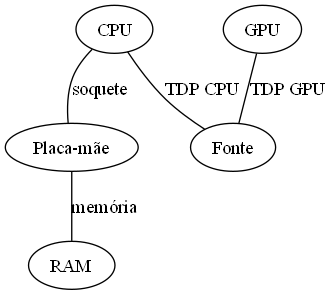
\includegraphics[width=0.5\textwidth]{imagens/grafo-restricoes.png}
  \\\textbf{Fonte:} Elaborada pelo autor
  \label{fig:grafo_restricoes}
\end{figure}
\FloatBarrier

% \FloatBarrier
% \begin{figure}[!htbp]
%   \centering
%   \caption{Grafo de Restrições do Sistema Proposto}
%   %scale redimensiona a figura.
%   %1.5 = 150% do tamanho original
%   %1 = 100% do tamanho original
%   %0.20 = 20% do tamanho original
%   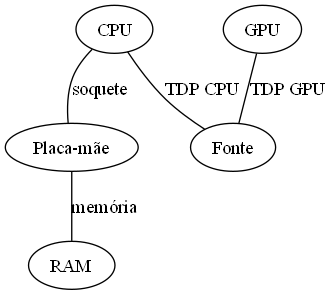
\includegraphics[scale=0.3]{imagens/grafo-restricoes.png}
%   \\\textbf{Fonte:} Elaborada pelo autor
%   \label{fig:exemplo}
% \end{figure}
% \FloatBarrier

Essa estrutura revela que a Fonte é um vértice de alta centralidade no grafo, pois está conectada tanto
à CPU quanto à GPU, de modo que qualquer alteração no domínio de um desses componentes pode propagar
restrições para o domínio da Fonte. A Placa-mãe, por sua vez, é o vértice que medeia a compatibilidade entre CPU e RAM,
funcionando como ponto de articulação da rede de restrições. Esse grafo é o objeto sobre o qual os algoritmos de busca
e propagação operam, cuja complexidade computacional é analisada na seção seguinte.

% ============================================================
\section{Complexidade Computacional}
\label{sec:complexidade}
% ============================================================

A teoria da complexidade computacional ocupa-se da classificação de problemas de decisão segundo
os recursos algorítmicos, principalmente tempo de execução e espaço de memória, exigidos para sua resolução \cite{Cormen2001}.
Dentro desse arcabouço, a classe P reúne os problemas para os quais existem algoritmos determinísticos
de tempo polinomial, considerados eficientes e tratáveis mesmo para entradas de grande escala.
A classe NP, por sua vez, abrange os problemas cuas soluções propostas podem ser verificados em tempo polinomial
por uma máquina determinística, ainda que não se conheça, até o presente, algoritmo eficiente para encontrá-las \cite{Sipser2012}.
A questão sobre a relação entre essas duas classes, se $P = NP$, permanece em aberto e constitui
o problema não resolvido de maior relevância para a ciência da computação teórica, razão pela qual o
\textit{Clay Mathematics Institute} o incluiu entre os sete Problemas do Milênio \cite{Sipser2012}.

O interior da classe NP não é uniforme. A literatura demonstra a existência de subclasses com diferentes
graus de dificuldade, incluindo problemas resolúveis em tempo subexponencial por meio de não-determinismo limitado \cite{Papadimitriou1996}.
O CSP, contudo, não se enquadra nessas classes intermediárias, situando-se no topo da hierarquia como um problema NP-completo \cite{Sipser2012}.
Um problema é classificado como NP-completo quando pertence a NP e todo problema NP se reduz
a ele em tempo polinomial, essa classificação pode ser estabelecida por redução polinomial a partir
do Problema da Satisfabilidade Booleana (SAT), um dos problemas canônicos de NP-completude \cite{Cormen2001,Sipser2012}.
Consequentemente, se qualquer problema NP-completo admitisse solução em tempo polinomial,
toda classe NP colapsaria em P \cite{Sipser2012}.

\subsection{Implicações para o Domínio de Hardware}
Essa natureza NP-completa impõe restrições severas à arquitetura de qualquer sistema de verificação
de compatibilidade de \textit{hardware} fundamentado em CSP. A primeira limitação é de ordem temporal,
a avaliação exaustiva de todas as combinações interdependentes de componentes é inviável na prática em razão
da explosão combinatória intrínseca à classe \cite{Sipser2012,Cormen2001}. Para ilustrar concretamente, considere
que cada categoria de componente possui em média 50 modelos disponíveis no catálogo do sistema. Com cinco
categorias (CPU, Placa-mãe, RAM, GPU e Fonte), a avaliação por força bruta implicaria examinar $50^5 = 312.500.000$ atribuições
candidatas antes de encontrar uma solução válida no pior caso. Esse número cresce exponencialmente à medida
que o catálogo se expande, tornando a abordagem inviável em tempo hábil.

A segunda limitação é de ordem espacial, estratégias alternativas baseadas no mapeamento
estático e exaustivo de regras lógicas condicionais, codificando explicitamente cada restrição de \textit{hardware}
por meio de estruturas if-else ou tabela de decisão, não contornam o problema, pois a representação de funções
lógicas complexas por árvores de decisão pode exiger espaço de tamanho exponencial \cite{Jukna1999}. Diante
dessas limitações, a abordagem padrão para tornar CSPs tratáveis na prática é a busca sistemática
com retrocesso combinada com técnicas de propagação de restrições, que reduzem o espaço efetivo
de busca de forma incremental.

\section{Algoritmos de Busca e Backtracking}
\label{sec:backtracking}

\subsection{Busca em Espaço de Atribuições}
Dado o grafo de restrições e a complexidade NP-completa do CSP, é necessário um algoritmo
de busca sistemática que explore o espaço de atribuições de forma inteligente,
sem enumerar cegamente todas as combinações possíveis. O ponto de partida é o conceito
de atribuição parcial, uma função que associa valores a um subconjunto das variáveis,
podendo ser progressivamente estendida até uma atribuição completa \cite{Russell2010}.
A ideia central dos algoritmos de busca para CSP é construir a atribuição incrementalmente,
verificando consistência a cada passo e abandonando ramos da árvore de busca assim que
uma inconsistência é detectada.

\subsection{Backtracking}
O algoritmo de \textit{backtracking} é o método fundamental de busca para CSPs \cite{Russell2010,Kumar1992}.
Ele percorre recursivamente a árvore de atribuições, em cada nível da recursão, seleciona uma variável
ainda não atribuída, tenta cada valor do seu domínio na ordem disponível, verifica se esse valor é consistente
com as restrições envolvendo as variáveis já atribuídas e recua (\textit{backtrack}) ao encontrar uma inconsistência.
O pseudocódigo do algoritmo é apresentado a seguir:

\begin{algorithm}[hbtp]
  \caption{Algoritmo de Busca por Backtracking para CSP}\label{alg:backtracking}
  \vspace{2mm} % Dá um respiro entre o título e a linha
  \hrule % Desenha a linha superior
  \vspace{2mm} % Dá um respiro entre a linha e o código

  \begin{algorithmic}[1]
    \Function{Backtracking-Search}{$csp$}
    \State \Return \Call{Backtrack}{$\emptyset, csp$}
    \EndFunction
    \Statex
    \Function{Backtrack}{$atribuicao, csp$}
    \If{$atribuicao$ está completa}
    \State \Return $atribuicao$
    \EndIf
    \State $var \gets$ \Call{Selecionar-Variavel-Nao-Atribuída}{$csp$}
    \ForAll{$valor$ em \Call{Ordenar-Valores}{$var, atribuicao, csp$}}
    \If{$valor$ é consistente com $atribuicao$ dado $csp$}
    \State adicionar $\{var = valor\}$ à $atribuicao$
    \State $resultado \gets$ \Call{Backtrack}{$atribuicao, csp$}
    \If{$resultado \neq$ falha}
    \State \Return $resultado$
    \EndIf
    \State remover $\{var = valor\}$ da $atribuicao$
    \EndIf
    \EndFor
    \State \Return falha
    \EndFunction
  \end{algorithmic}

  \vspace{2mm}
  \hrule % Desenha a linha inferior
  \vspace{2mm}
  \fonte{Adaptado de: \textcite{Russell2010}} % Adiciona a fonte padrão ABNT. Se o comando \fonte der erro no seu template, use apenas: Fonte: O autor (2026).
\end{algorithm}


A complexidade de pior caso do \textit{backtracking} puro é $O(d^n)$, na qual $d$ é o tamanho
máximo dos domínios e $n$ é o número de variáveis, reiterando a inviabilidade para instâncias grandes
sem otimizações complementares \cite{Russell2010}.

\subsection{Forward Checking}
Uma primeira melhoria ao backtracking puro é o \textit{forward checking} \cite{Dechter2003}.
Ao atribuir um valor à variável $X_i$, o algoritmo imediatamente examina cada variável $X_j$, ainda
não atribuída que compartilha uma restrição com $X_i$ e remove de $Dom(X_j)$ todos os valores que se tornam
inconsistentes com a atribuição de $X_i$. Se algum domínio $X_j$ se torna vazio, o algoritmo detecta
a falha antecipadamente e recua, sem precisar explorar o ramo até o fim.

Aplicando ao domínio de \textit{hardware}, ao selecionar uma CPU com soquete AM5,
o \textit{forward checking} percorre os vizinhos de CPU no grafo de restrições e remove do domínio
de Placa-mãe todos os modelos com soquete incompatível com AM5, antes mesmo de tentar atribuir um valor
a Placa-mãe. Essa poda antecipada reduz significativamente o número de atribuições exploradas.
Contudo, o \textit{forward checking} verifica apenas os vizinhos diretos da variável recém-atribuída,
sem propagar as consequências dessas remoções para variáveis mais distantes no grafo. A forma mais
completa e eficiente de propagação, que garante consistência global na rede, é o Algoritmo AC-3.

\section{Propagação de Restrições e Algoritmo AC-3}
\label{sec:ac3}
A principal técnica para contornar a explosão combinatória é a propagação de restrições,
realizada por algoritmos de consistência. O mais consolidado na literatura é o AC-3
(\textit{Arc Consistency Algorithm 3}), proposto por \cite{Mackworth1977}, cujo objetivo é garantir
a consistência de arco em redes de restrições binárias \cite{Kumar1992}. Diz-se que um arco
$(X_i, X_j)$ é consistente quando, para todo valor $v \in Dom(X_i)$, existe ao menos um valor
$w \in Dom(X_j)$ tal que a atribuição ${X_i = v, X_j = w}$ satisfaz a restrição entre as duas variáveis.

O algoritmo mantém uma fila de arcos a examinar e, para cada par de variáveis relacionadas,
remove do domínio da variável os valores que não encontram suporte em nenhum valor do domínio da
variável vizinha. Cada remoção dispara a reinserção dos arcos afetados na fila, propagando
a mudança pela rede até o ponto de estabilidade, em que nenhuma redução adicional é possível \cite{Russell2010}.
Assumindo um CSP com $n$ variáveis, domínios de tamanho máximo $d$ e $c$ restrições binárias, a complexidade
de pior caso do AC-3 é $O(cd^3)$ \cite{Russell2010}.

\subsection{Aplicação ao Domínio de Hardware}
Para ilustrar a execução do AC-3 no sistema proposto, considera-se o cenário
em que o usuário seleciona um processador com soquete AM5. A Figura~\ref{fig:ac3_execucao}
apresenta os quatro passos da execução do algoritmo sobre o grafo de restrições
formado pelas variáveis Processador e Placa-mãe.

\FloatBarrier
\begin{figure}[!htbp]
  \centering
  \caption[Execução do AC-3]{Execução passo a passo do AC-3 no grafo de hardware}
  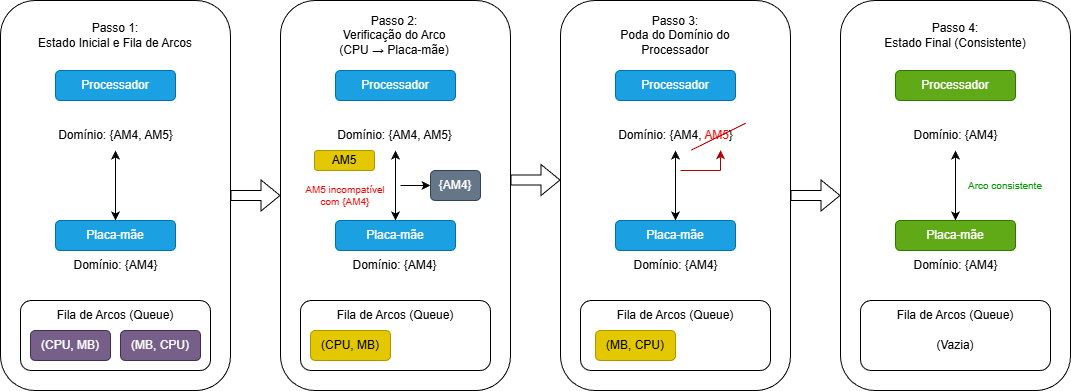
\includegraphics[width=1\textwidth]{imagens/execucao-passo-a-passo-ac-3 (2).png}
  \\\textbf{Fonte:} Elaborada pelo autor
  \label{fig:execucao_ac3}
\end{figure}
\FloatBarrier

No \textbf{Passo 1}, o estado inicial é estabelecido: o domínio do Processador
contém dois valores, AM4 e AM5, e o domínio da Placa-mãe contém apenas AM4.
A fila de arcos é inicializada com os dois arcos direcionados da restrição
bínária: (CPU, MB) e (MB, CPU).

No \textbf{Passo 2}, o arco (CPU, MB) é retirado da fila para verificação.
O algoritmo examina cada valor do domínio do Processador e verifica se existe,
no domínio da Placa-mãe, ao menos um valor que satisfaça a restrição de soquete.
Para o valor AM4, existe suporte no domínio da Placa-mãe. Para o valor AM5,
não existe suporte, pois a placa disponível suporta apenas AM4 --- a incompatibilidade
é identificada.

No \textbf{Passo 3}, o valor AM5 é removido do domínio do Processador por não
possuir suporte na variável vizinha. O arco (MB, CPU) é reinserido na fila para
que o algoritmo verifique se as remoções realizadas tornaram algum valor da
Placa-mãe inconsistente.

No \textbf{Passo 4}, o arco (MB, CPU) é processado. O valor AM4 da Placa-mãe
encontra suporte no valor AM4 do Processador, portanto nenhuma remoção adicional
é necessária. A fila esvazia e o algoritmo encerra no ponto de estabilidade:
ambas as variáveis possuem domínios consistentes com a restrição, sem necessidade
de explorar nenhuma atribuição completa por força bruta.

O resultado ilustra o mecanismo central do motor de inferência: uma única seleção
do usuário dispara a propagação de restrições por toda a rede, reduzindo os
domínios disponíveis de forma incremental e em tempo real \cite{Mackworth1977,Russell2010}.

\section{Sistema Especialista}
\label{sec:sistema-especialista}
Um Sistema Especialista (SE) é um programa de computador projetado para simular o raciocínio de um
especialista humano em um domínio restrito e bem definido \cite{Russell2010}. Diferentemente de sistema
de propósito geral, um SE concentra seu conhecimento em um domínio específico e é capaz de resolver
problemas nesse domínio com nível de competência comparável ao de um especialista humano \cite{Jackson1998}.
Sua arquitetura é composta por três elementos centrais: a base de conhecimento, que armazena fatos
e regras sobre o domínio, o motor de inferência, que aplica essas regras aos fatos disponíveis
para derivar conclusões e a interface de explicação, que permite ao sistema justificar
suas respostas ao usuário \cite{Russell2010}.

O motor de inferência pode operar segundo encadeamento progressivo (\textit{forward chaining}),
partindo dos fatos conhecidos em direção a conclusões, ou encadeamento regressivo (\textit{backward chaining}),
partindo de uma hipótese e verificando se os fatos disponíveis a sustentam \cite{Russell2010}.
No sistema proposto, o motor opera predominantemente em modo progressivo: a cada seleção de componente
pelo usuário, o sistema propaga as restrições a partir desse novo fato para derivar quais opções
permanecem válidas.

\subsection{Explanation Facilities}
A capacidade de justificar o próprio raciocínio, denominada na literatura como
\textit{explanation facility}, é o que distingui fundamentalmente um SE de um mecanismo
de filtragem comum \cite{Clancey1983}. Segundo \cite{Clancey1983}, essa capacidade exige que o sistema
mantenha não apenas as conclusões derivadas, mas também a cadeia de regras e restrições que
levou a cada conclusão, de modo que possa reconstruir e comunicar o raciocínio em linguagem
acessível ao usuário. Um mecanismo de filtragem simples responde apenas à pergunta "quais opções são válidas?",
apresentado resultados sem elaboração. Um SE com \textit{explanation facility} responde também à pergunta
"por que as demais opçõs são inválidas?", articulando a regra específica que foi violada.

No contexto do sistema proposta, essa capacidade se manifesta da seguinte forma, ao bloquear a seleção de um módulo DDR4 após
a escolha de uma CPU AM5, o sistema não se limita a remover o componente da lista de opções,
ele apresenta ao usuário uma justificativa explícita como "Este módulo de memória é incompatível: a placa-mãe
compatível com o processador selecionada suporta exclusivamente DDR5 e este módulo é DDR4". Essa explicação
transforma cada bloqueio em uma oportunidade de aprendizado sobre as restrições físicas do \textit{hardware}.

\subsection{Inteligência Artificial Explicável (XAI)}
O problema identificado por \textcite{Clancey1983}, a necessidade de sistemas inteligentes justificarem seu
raciocónio ao usuário, permaneceu latente por décadas e ressurgiu com força renovada no contexto da Inteligência Artificial (IA)
moderna sob o nome de XAI (\textit{eXplainable Artificial Intelligence}), ou Inteligência Artificial Explicável. \textcite{Arrieta2020}
definem XAI como o conjunto de processos e técnicas que permitem que modelos de inteligência artificial produzam
resultados compreensíveis por seres humanos, especialmente por usuários finais sem formação técnica em IA.
Os autores identificam a explicabilidade como uma necessidade crítica para a adoção prática de sistemas de IA em domínios
sensíveis, argumentando que um sistema que apenas produz resultados sem justificá-los não gera confiança suficiente para
ser adotado em decisões reais.

A distinção central que o campo de XAI estabelece é entre sistemas caixa-preta (\textit{black-box}), cujo processo
de decisão interno é opaco ao usuário, e sistemas transparentes, cujo raciocínio pode ser inspecionado e compreendido \cite{Arrieta2020}.
Sistemas especialistas baseados em CSP pertencem naturalmente à segunda categoria, as variáveis, os domínios e as restrições
são explícitos e auditáveis e cada decisão de bloqueio pode ser rastreada até a restrição específica que a originou.
Nesse sentido, o motor de inferência CSP/AC-3 proposto neste trabalho é intrinsecamente explicável por \textit{design}, não por
técnica de pós-processamento, mas pela própria natureza simbólica do modelo. Isso posiciona o sistema proposto em alinhamento com
os princípios contemporâneos de XAI, cada resultado produzido pelo motor de inferência é acompanhado da justificativa técnica
que o fundamenta, tornando o processo de validação de \textit{hardware} transparente e auditável pelo usuário.

\subsection{Mapeamento ao Sistema Proposto}
O sistema proposto neste trabalho se enquadra na categoria de sistemas especialistas baseados em restrições.
Os três componentes arquiteturais do SE mapeiam diretamente à implementação: a base de conhecimento corresponde
à camada de dados que armazena as especificações técnicas dos componentes e as regras de compatibilidade modeladas
como restrições do CSP; o motor de inferência corresponde ao algoritmo AC-3 implementado na camada de lógica da aplicação,
responsável por propagar restrições e podar domínios a cada interação do usuário; e a interface de explicação corresponde
aos alertas técnicos e educativos exibidos na camada de apresentação, que comunicam ao usuário não apenas quais componentes
são bloqueados, mas as razões físicas e técnicas subjacentes a cada bloqueio \cite{Jackson1998}.

\section{Dimensão Educativa em Sistemas Especialistas}
\label{sec:dimensao-educativa}
O caráter educativo do sistema proposto não decorre da adoção de uma arquitetura de aprendizagem  adaptativa,
mas da forma como o motor de inferência comunica suas conclusões ao usuário. Para delimitar com precisão
essa dimensão, é necessário distinguir três categorias de sistemas que operam sobre domínios de conhecimento restrito:
os mecanismos de filtragem, os Sistemas Tutores Inteligentes (STI) e os Sistemas Especialistas com interface educativa.


\subsection{Mecanismo de Filtragem versus Sistema com Explicação}
Um mecanismo de filtragem tradicional opera sobre um conjunto de dados e retorna os elementos que
satisfazem determinados critérios, sem qualquer elaboração sobre o processo de decisão. No contexto de compatibilidade de
\textit{hardware}, um filtro responde à pergunta "quais componentes são compatíveis com minha seleção atual?", apresentando
uma lista de resultados válidos e ocultando ou desabilitando os inválidos, sem indicar o motivo da exclusão. Plataformas comerciais
como o \textit{PC Part Picker} operam predominantemente nesse paradigma: informam a incompatibilidade, mas raramente
explicam a regra física que a origina.

A limitação pedagógica desse modelo é nítida: o usuário aprende o que não pode fazer, mas não aprende o motivo.
Cada bloqueio silencioso é uma oportunidade de aprendizagem perdida \cite{Clancey1983}. Um sistema que apenas
filtra não transfere conhecimento, apenas restringe escolhas.

\subsection{Sistemas Tutores Inteligentes}
Sistemas Tutores Inteligentes (STI) representam o paradigma mais sofisticado de instrução mediada por computador.
Sua arquitetura formal é composta por quatro modelos interdependentes: o modelo de domínio, que representa o
conhecimento a ser ensinado; o modelo de estudante, que representa o estado de conhecimento individual do aprendiz e é
atualizado continuamente com base em seus erros e acertos; o modelo pedagógico, que define as estratégias de instrução e adaptação;
e o modelo da interface, que define como o conteúdo é apresentado \cite{Woolf2008}. O elemento central que distingue
um STI de outros sistemas é o modelo de estudante, ele exige que o sistema mantenha um perfil persistente por usuário, rastreando o histórico
de interações ao longo de múltiplas sessões para personalizar a instrução \cite{Anderson1995}.

O sistema proposto neste trabalho não implementa a arquitetura de um STI. Não há rastreamento de sessões individuais,
não há perfil persistente de usuário e não há adaptação sequencial de conteúdo baseado em histórico. Essa delimitação
é intencional, pois o objetivo é criar um sistema especialista com interface educativa, que se concentra na explicação
de cada bloqueio como uma oportunidade de aprendizagem, sem a complexidade adicional de um modelo de estudante adaptativo.

\subsection{Sistema Especialista Educacional}
O sistema proposto se enquadra na categoria de Sistema Especialista Educacional, um SE dotado de \textit{explanation facility}
cuja interface é projetado com objetivo pedagógico explícito. A distinção em relação a um SE convencional reside na forma como
as conclusões são comunicadas. Enquanto um SE padrão pode simplesmente retornar um resultado binário (compatível ou incompatível),
um SE educacional articula a cadeia de raciocínio que levou aquela conclusão em linguagem acessível ao usuário \cite{Clancey1983,Jackson1998}.

No sistema proposto, essa dimensão educativa se manifesta de forma precisa e delimitada: ao detectar uma violação de restrição
via propagação AC-3, o sistema não limita a bloquear o componente incompatível, ele apresenta ao usuário uma justificativa explícita
que identifica qual restrição foi violada e por qual razão técnica. Por exemplo, ao tentar selecionar um módulo DDR4 após escolher
umas CPU com plataforma AM5, o sistema exibe: "Este módulo de memória é incompatível: a placa-mãe compatível com o processador selecionado
suporta exclusivamente DDR5, e este módulo utiliza o padrão DDR4". Essa explicação transforma cada bloqueio em uma oportunidade de
aprendizagem sobre os princípios físicos que regem a montagem de computadores, sem requerer qualquer cadastro, histórico ou personalização
por parte do usuário.

Essa abordagem é pedagogicamente coerente com público-alvo do sistema, o usuário leigo que realiza uma única sessão de configuração,
para quem a explicação contextualizada e imediata é mais eficaz do que qualquer mecanismo de adaptação baseado em histórico. O adjetivo
"Educacional" no título do trabalho refere-se precisamente a essa capacidade de instruir o usuário sobre as restrições do domínio no exato
momento em que elas se tornam relevantes para sua decisão.

\section{Arquitetura de Software Orientada a Serviços}
\label{sec:arquitetura-software}

\subsection{Arquitetura em Camadas}
A arquitetura de \textit{software} compreende o conjunto de decisões estruturais fundamentais que definem a organização
de um sistema, as responsabilidades de seus componentes e as interfaces através das quais eles se comunicam \cite{Fowler2002}.
Um dos padrões arquiteturais mais consolidados na engenharia de \textit{software} é a arquitetura em camadas, que organiza
o sistema em níveis hierárquicos de abstração, cada um com responsabilidades bem delimitadas e comunicando-se apenas com
a camada imediatamente adjacente \cite{Fowler2002}.

As três camadas clássicas são: a camada de apresentação, responsável pela interação com o usuário e pela exibição de informações,
a camada de lógica de negócio, responsável pelo processamento, pelas regras do domínio e pelas decisões da aplicação e a camada de dados,
responsável pelo armazenamento, recuperação e persistência de informações \cite{Fowler2002}. Essa separação aumenta a manutenibilidade
do sistema, alterações em uma camada não propagam mudanças para as demais, e facilita a testabilidade, permitindo que cada camada seja
verificada de forma independente.

\subsection{REST como Estilo Arquitetural}
A comunicação entre camadas distribuídas em sistemas \textit{web} segue estilos arquiteturais que impõem restrições sobre
como os componentes interagem. O estilo mais amplamente adotado é o REST (\textit{Representational State Transfer}), definido por
\cite{Fielding2000} em sua tese de doutorado como um conjunto de seis princípios arquiteturais para sistemas distribuídos baseados
em rede.

Os princípios mais relevantes para o sistema proposto são:

O princípio de cliente-servidor, que estabelece a separação entre a interface do usuário e o armazenamento e processamento de dados,
permitindo que cada lado evolua de forma independente. No sistema proposto, o cliente e o servidor evoluem independentemente, a interface
pode ser redesenhada sem alterar o motor CSP, e o motor CSP pode ser otimizado sem alterar a inteface.

O princípio \textit{stateless} (sem estado), que estabelece que cada requisição enviado pelo cliente ao servidor deve conter
todas as informações necessárias para ser compreendida e processada, sem depender de contexto ou sessão armazenada no servidor
entre requisições \cite{Fielding2000}. No contexto do sistema proposto, isso significa que cada chamada à \textit{API} carrega o
estado atual completo das seleções do usuário, quais componentes foram escolhidos e quais permanecem em aberto e o motor CSP
executa a propagação de restrições a partir desse estado, sem manter sessão persistente no servidor. Essa característica garante
escalabilidade e simplicidade operacional.

O princípio da interface uniforme, que estabelece que a comunicação entre o cliente e servidor deve seguir um contrato padronizado,
baseado em recursos identificados por URIs e operações semânticas bem definidas \cite{Richardson2007}. No sistema proposto,
cada categoria de componente e cada conjunto de restrições é exposto como um recurso REST, acessível por operações HTTP padronizadas.

\subsection{Mapeamento ao Sistema Proposto}
A arquitetura do sistema proposto realiza concretamente os princípios da
arquitetura em camadas e do estilo REST, conforme ilustrado na
Figura~\ref{fig:arquitetura_rest}.

\FloatBarrier
\begin{figure}[!htbp]
  \centering
  \caption[Diagrama da arquitetura em três camadas do sistema]{Diagrama da arquitetura em três camadas do sistema}
  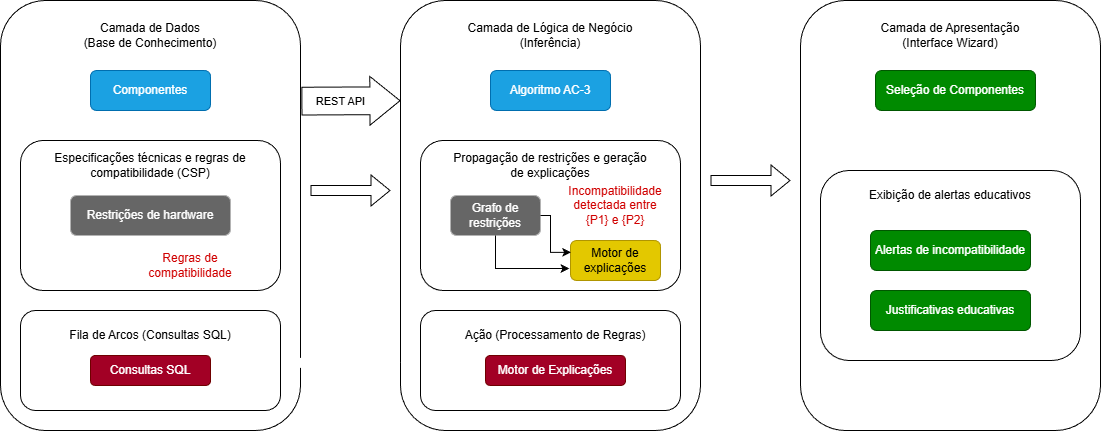
\includegraphics[width=1\textwidth]{imagens/DIAGRAMA REST.png}
  \\\textbf{Fonte:} Elaborada pelo autor
  \label{fig:diagrama_arquitetura}
\end{figure}
\FloatBarrier

A \textbf{camada de dados}, representada no painel esquerdo da figura, armazena
a base de conhecimento do sistema especialista: os modelos de componentes de
\textit{hardware}, as especificações técnicas que constituem as variáveis do CSP,
as restrições de compatibilidade que compõem o conjunto $C$, e as regras de
compatibilidade que fundamentam as decisões do motor de inferência. O acesso
a essa camada é realizado por meio de consultas SQL disparadas pela camada
de lógica de negócio.

A \textbf{camada de lógica de negócio}, representada no painel central, é o
núcleo inteligente do sistema. Após receber uma requisição via \textit{REST API}
contendo o estado atual das seleções do usuário, essa camada executa o
Algoritmo AC-3 sobre o grafo de restrições: identifica os arcos inconsistentes,
poda os domínios das variáveis afetadas e, ao detectar uma incompatibilidade
entre dois componentes $P_1$ e $P_2$, aciona o motor de explicações, que
formula a justificativa técnica a ser apresentada ao usuário. O resultado
do processamento é retornado à camada de apresentação como resposta à
requisição REST.

A \textbf{camada de apresentação}, representada no painel direito, é a interface
\textit{wizard} com a qual o usuário interage diretamente. Ela é responsável
por exibir o catálogo de componentes disponíveis para seleção, apresentar os
alertas de incompatibilidade gerados pelo motor de inferência e comunicar as
justificativas educativas que fundamentam cada bloqueio, transformando o
resultado da validação CSP em uma oportunidade de aprendizagem sobre os
princípios físicos que regem a montagem de computadores.

A separação entre as três camadas garante que o motor de inferência possa ser
mantido e expandido de forma independente da interface de apresentação,
preservando a modularidade arquitetural ao longo do ciclo de desenvolvimento
do sistema \cite{Fowler2002,Fielding2000}.

\section{Trabalhos Relacionados}
Esta seção mapeia o estado da arte em duas frentes: as plataformas comerciais de verificação de compatibilidade
de \textit{hardware} atualmente disponíveis e os trabalhos acadêmicos sobre sistemas especialistas e CSP aplicados
a domínios similares. O objetivo é evidenciar as lacunas existentes nas soluções atuais e posicionar a contribuição do
presente trabalho em relação a elas.

\subsection{Plataformas Comerciais de Compatibilidade de Hardware}
O PC Part Picker é a plataforma de referência global para montagem de computadores. Permite ao usuário
selecionar componentes de um catálogo extenso e verifica automaticamente incompatibilidades entre as pelas
escolhidas \cite{PCPARTPICKER2024}. Quando uma incompatibilidade é detectada, a plataforma exibe um alerta
genérico indicando que os componentes são incompatíveis, mas sem detalhar a regra técnica violada, por exemplo, ao selecionar uma
CPU AM5 com um módulo DDR4, o sistema indica o conflito sem explicar a diferença entre os padrões de memória
ou a razão física da incompatibilidade. Do ponto de vista da teoria de sistemas especialistas, o PC Part Picker
implementa um mecanismo de filtragem sem \textit{explanation facility}, o usuário recebe o resultado da
validação, mas não o raciocínio que o produziu \cite{Clancey1983}.

O Meupc.net é a alternativa nacional mais utilizada no contexto brasileiro, operando de forma similar
ao PC Part Picker com catálogo voltado ao mercado local \cite{MEUPC2024}. Apresenta as mesmas limitações
em termos de explicação, as incompatibilidades são sinalizadas visualmente, mas sem justificativa técnica que
permita ao usuário compreender o princípio de \textit{hardware} subjacente à restrição.

A limitação comum a ambas as plataformas é estrutural, por operaram como mecanismos de filtragem e não
como sistemas especialistas com capacidade explicativa, não transferem conhecimento ao usuário, apenas
restringem escolhas. Um usuário que utiliza PC Part Picker repetidamente aprende quais componentes são
compatíveis entre si, mas não aprende por que são compatíveis, o que o impede de generalizar
o conhecimento adquirido para novas situações de compra.

\subsection{Trabalhos Acadêmicos Relacionados}
Na literatura acadêmica, a aplicação de CSPs a problemas de configuração de produtos é um tema consolidado.
\textcite{Sabin1998} apresentam uma \textit{survey} abrangente sobre sistemas de configuração baseados em CSP,
identificando a modelagem de dependências entre componentes como variáveis e restrições é a abordagem mais
expressiva para domínios com regras de compatibilidade complexas. Os autores demonstram que sistemas de configuração
baseada em CSP superam abordagem baseadas em regras estáticas tanto em expressividade quanto em eficiência de
manutenção de base de conhecimento, resultado diretamente aplicável ao domínio de \textit{hardware} proposto neste trabalho.

\textcite{Mittal1989} introduzem o conceito de \textit{dynamic CSP}, no qual o conjunto de variáveis e restrições
pode ser alterado durante a busca, uma extensão relevante para sistemas de configuração interativos onde o
usuário faz escolhas incrementais, como é o caso do sistema proposto. Essa abordagem sustenta a decisão arquitetural
de propagar restrições a cada interação do usuário, em vez de processar o CSP completo apenas ao final da configuração.

No campo de sistemas especialistas educacionais, \textcite{Nwana1990} discute os requisitos para que um sistema
especialista seja considerado efetivamente educativo, identificando a capacidade de explicação como condição necessária,
mas não suficiente, para a transferência de conhecimento. O autor distingue sistemas que explicam o que de sistemas
\textit{o que} explicam \textit{por que}, argumentando que apenas os últimos têm impacto pedagógico real. Esse
referencial sustenta diretamente a decisão de projeto de exibir não apenas o resultado da validação, mas a regra de
compatibilidade violada em linguagem acessível ao usuário.

Mais recentemente, \textcite{Wang2018} desenvolveram um sistema especialista educacional para apoio ao aprendizado
de classificação botânica em ambiente móvel, demonstrando que sistemas especialistas com \textit{feedback} explicativo
produzem ganhos mensuráveis de aprendizagem em comparação com sistemas que apenas apresentam informação estática.
O estudo é relevante para o presente trabalho por demonstrar empiricamente que a capacidade de explicação, e não
apenas a apresentação de conteúdo, é o fator determinante para o impacto pedagógico de um sistema especialista,
validando a abordagem adotada no sistema de compatibilidade de \textit{hardware} proposto.

\subsection{Posicionamento do Trabalho Proposto}
A análise das plataformas comerciais e dos trabalhos acadêmicos permite identificar com precisão a contribuição do presente
trabalho. Em relação as plataformas comerciais, o diferencial está na \textit{explanation facility}. enquanto PC Part Picker
e Meupc.net sinalizam incompatibilidades sem explicá-las, o sistema proposto articula a regra técnica violada em cada bloqueio,
transformando a interação em uma oportunidade de aprendizagem. Em relação aos trabalhos acadêmicos, a contribuição está na combinação
de três elementos que, individualmente, já são estudados na literatura, CSP como motor de inferência \cite{Sabin1998}, sistema
especialista com capacidade explicativa alinhada a princípios de XAI \cite{Clancey1983,Arrieta2020} e interface educativa
com impacto pedagógico demonstrável \cite{Wang2018}, em um sistema \textit{web} completo validado sobre um domínio concreto
e de relevância prática imediata para o usuário.

% Texto da revisão da literatura, dividido em seções e subseções.


% Este é um exemplo de como usar figuras. Referência cruzada: Figura~\ref{fig:exemplo}

% \FloatBarrier
% \begin{figure}[!htbp]
%   \centering
%   \caption{Exemplo de figura}
%   %scale redimensiona a figura.
%   %1.5 = 150% do tamanho original
%   %1 = 100% do tamanho original
%   %0.20 = 20% do tamanho original
%   
\includegraphics[scale=0.3]{imagens/LogoIF_BRI10}
%   \\\textbf{Fonte:} Elaborada pelo autor
%   \label{fig:exemplo}
% \end{figure}
% \FloatBarrier


% Este é um exemplo de como usar tabelas. Referência cruzada: Tabela~\ref{tab:exemplo}

% \FloatBarrier
% \begin{table}[!htbp]
%   \centering
%   \caption{Exemplo de tabela de 2 colunas}
%   \begin{tabular}{ c | c }
%     \hline
%     \textbf{Coluna 1} & \textbf{Coluna 2} \\ \hline
%     Dado 1a           & Dado 2a           \\ \hline
%     Dado 1b           & Dado 2b           \\ \hline
%     Dado 1c           & Dado 2c           \\ \hline
%     Dado 1d           & Dado 2d           \\ \hline
%   \end{tabular}
%   \\ \vspace{0.2cm}
%   \textbf{Fonte:} Elaborada pelo autor
%   \label{tab:exemplo}
% \end{table}
% \FloatBarrier


% Este é um exemplo de como usar quadros. Referência cruzada: Quadro~\ref{qua:exemplo}

% \FloatBarrier
% \begin{quadro}[!htbp]
%   \centering
%   \caption{Exemplo de quadro}
%   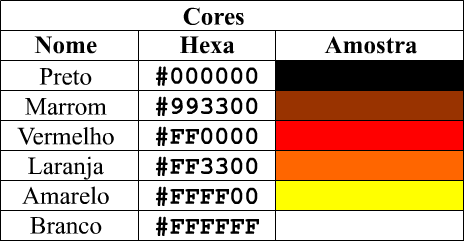
\includegraphics[scale=.7]{imagens/exemploQuadro}
%   \\\textbf{Fonte:} Elaborada pelo autor
%   \label{qua:exemplo}
% \end{quadro}
% \FloatBarrier


% Este é um exemplo de como usar equações. Referência cruzada: Equação~\ref{eq:exemplo}

% \begin{equation}
%   \sum_{i=1}^{n} i = \frac{n(n+1)}{2}
%   \label{eq:exemplo}
% \end{equation}


% Exemplo de inserção de lista de código fonte (\textbf{\textcolor{red}{não use acentos no código!}}):

% \lstinputlisting[language=Java]{fontes/ClasseExemplo.java}



% Este é um exemplo de como inserir texto sem formatação (ambiente verbatim):

% \begin{verbatim}
% 	Texto sem formatação, como espaçamento igual.
% \end{verbatim}


% Exemplo de lista de itens:

% \begin{itemize}
%   \item \textbf{Item 1:} texto...;
%   \item \textbf{Item 2:} texto...;
%         \begin{itemize}
%           \item \textbf{Subitem:} texto...;
%           \item \textbf{Subitem:} texto...;
%           \item \textbf{Subitem:} texto...;
%         \end{itemize}
%   \item \textbf{Item 3:} texto...;
%   \item \textbf{Item n:} texto....
% \end{itemize}


% Exemplo de lista numerada:

% \begin{enumerate}
%   \item \textbf{Item:} texto...;
%   \item \textbf{Item:} texto...;
%         \begin{enumerate}
%           \item \textbf{Subitem:} texto...;
%           \item \textbf{Subitem:} texto...;
%           \item \textbf{Subitem:} texto...;
%         \end{enumerate}
%   \item \textbf{Item:} texto...;
%   \item \textbf{Item:} texto....
% \end{enumerate}


% Exemplos de comandos para texto e referências:

% \begin{itemize}
%   \item Para iniciar um novo parágrafo, basta deixar uma linha em branco no código fonte;
%   \item Não force o compilador a pular mais de uma linha, pois terá influência negativa na composição do documento;
%   \item Sempre deixe o \LaTeX\ realizar a formatação de parágrafos e posicionamento de elementos;
%   \item Utilização de aspas simples (abertura \verb|`|, fechamento \verb|'|): `Texto entre aspas simples';
%   \item Utilização de aspas duplas (abertura \verb|``|, fechamento \verb|''|): ``Texto entre aspas duplas'';
%   \item Negrito (comando \verb|\textbf|): \textbf{texto em negrito};
%   \item Itálico (comando \verb|\textit|): \textit{texto em itálico};
%   \item Sublinhado (comando \verb|\underline|): \underline{texto sublinhado};
%   \item Negrito e itálico (usar comandos juntos): \textbf{\textit{texto em negrito e itálico}};
%   \item Alterar cor do texto (comando \verb|\textcolor{cor}{texto}|):
%         \begin{itemize}
%           \item Exemplo \verb|\textcolor{red}{texto}|: \textcolor{red}{texto vermelho};
%           \item Exemplo \verb|\textcolor[RGB]{255, 102, 0}|: \textcolor[RGB]{255, 102, 0}{texto laranja};
%           \item Exemplo \verb|\textcolor[HTML]{006AD7}|: \textcolor[HTML]{006AD7}{texto azul};
%         \end{itemize}
%   \item Ambiente matemático inline (comando \verb|$ expressão $|): $s = x^2-2x +1$;
%   \item Referência normal (comando \verb|\cite|):
%         \begin{itemize}
%           \item \cite{Agaisse1995};
%           \item \cite{Abedi2014};
%           \item \cite{BtNomenclature2016};
%         \end{itemize}
%   \item Referência normal com mais de uma obra (comando \verb|\cite|):
%         \begin{itemize}
%           \item \cite{Abedi2014, Agaisse1995};
%           \item \cite{AgapitoTenfen2014, BtNomenclature2016, Nelson2014};
%         \end{itemize}
%   \item Referência nome e ano (comando \verb|\citeauthorandyear|):
%         \begin{itemize}
%           \item \textcite{Agaisse1995};
%           \item \textcite{Abedi2014};
%           \item \textcite{BtNomenclature2016};
%         \end{itemize}
% \end{itemize}


% Exemplo 1 de citação direta:

% \begin{citacao}
%   Os 20 aminoácidos usualmente encontrados como resíduos em proteínas contém um grupo $\alpha$-carboxil, um grupo $\alpha$-amino e um grupo R distinto substituído no átomo de carbono $\alpha$. O átomo de carbono $\alpha$ de todos os aminoácidos, com exceção da glicina, é assimétrico e, portanto, os aminoácidos podem existir em pelo menos duas formas estereoisoméricas. Somente os estereoisômeros L, com uma configuração relacionada à configuração absoluta da molécula de referência L-gliceraldeído, são encontrados em proteínas \cite[p. 81]{Nelson2014}.
% \end{citacao}

% Exemplo 2 de citação direta:

% \begin{citacao}
%   \textit{These various insecticidal proteins are synthesized during the stationary phase and accumulate in the mother cell as a crystal inclusion which can account for up to 25\% of the dry weight of the sporulated cells. The amount of crystal protein produced by a B. thuringiensis culture in laboratory conditions (about 0.5 mg of protein per ml) and the size of the crystals (24) indicate that each cell has to synthesize $10^6$ to $2 \times 10^6$ $\delta$-endotoxin molecules during the stationary phase to form a crystal} \cite[p. 1]{Agaisse1995}.
% \end{citacao}

% Exemplo de nota de rodapé\footnote{Essa é uma nota de rodapé!}.